\documentclass[12pt, letterpaper]{memoir}
\usepackage{ExamStyle}

\begin{document}
	\pagestyle{empty}
	{\large Formulas}
	
	\begin{minipage}{0.5\linewidth}
		$\dfrac{rate_2}{rate_1}=\left(\dfrac{\left[ A\right]_2}{\left[ A\right]_1}\right)^m$
		
		$\dfrac{1}{[A]_t} = kt + \dfrac{1}{[A]_0}$
		
		$[A]_t=-kt+[A]_0$
		
		$t_{\nicefrac{1}{2}} = \dfrac{[A]_0}{2k}$
		
		$k=Ae^{\nicefrac{-E_a}{RT}}$
		
		$x=\dfrac{-b\pm\sqrt{b^2-4ac}}{2a}$
	\end{minipage}
	\begin{minipage}{0.5\linewidth}
		$\dfrac{[A]_t}{[A]_0}=\left(\dfrac{1}{2}\right)^{\dfrac{t}{t_{\nicefrac{1}{2}}}}$	
		
		$t_{\nicefrac{1}{2}}=\dfrac{\ln{2}}{k}$
		
		$\ln[A]_t=-kt+\ln[A]_0$
		
		$t_{\nicefrac{1}{2}} = \dfrac{1}{k[A]_0}$
			
		$\ln\left(\dfrac{k_2}{k_1}\right)=\dfrac{-E_a}{R}\left(\dfrac{1}{T_2}-\dfrac{1}{T_1}\right)$
		
		$K_P=K_C\left(RT\right)^{\Delta n}$
	\end{minipage}
	
	\vspace{2em}

	{\large Constants}
	
	$R=8.314 \dfrac{J}{mol~K}$
	
	$R=0.08206 \dfrac{L~atm}{mol~K}$
	

	
    \newgeometry{top=1mm, bottom=1mm, left=1mm, right=1mm}


\hspace{6em}	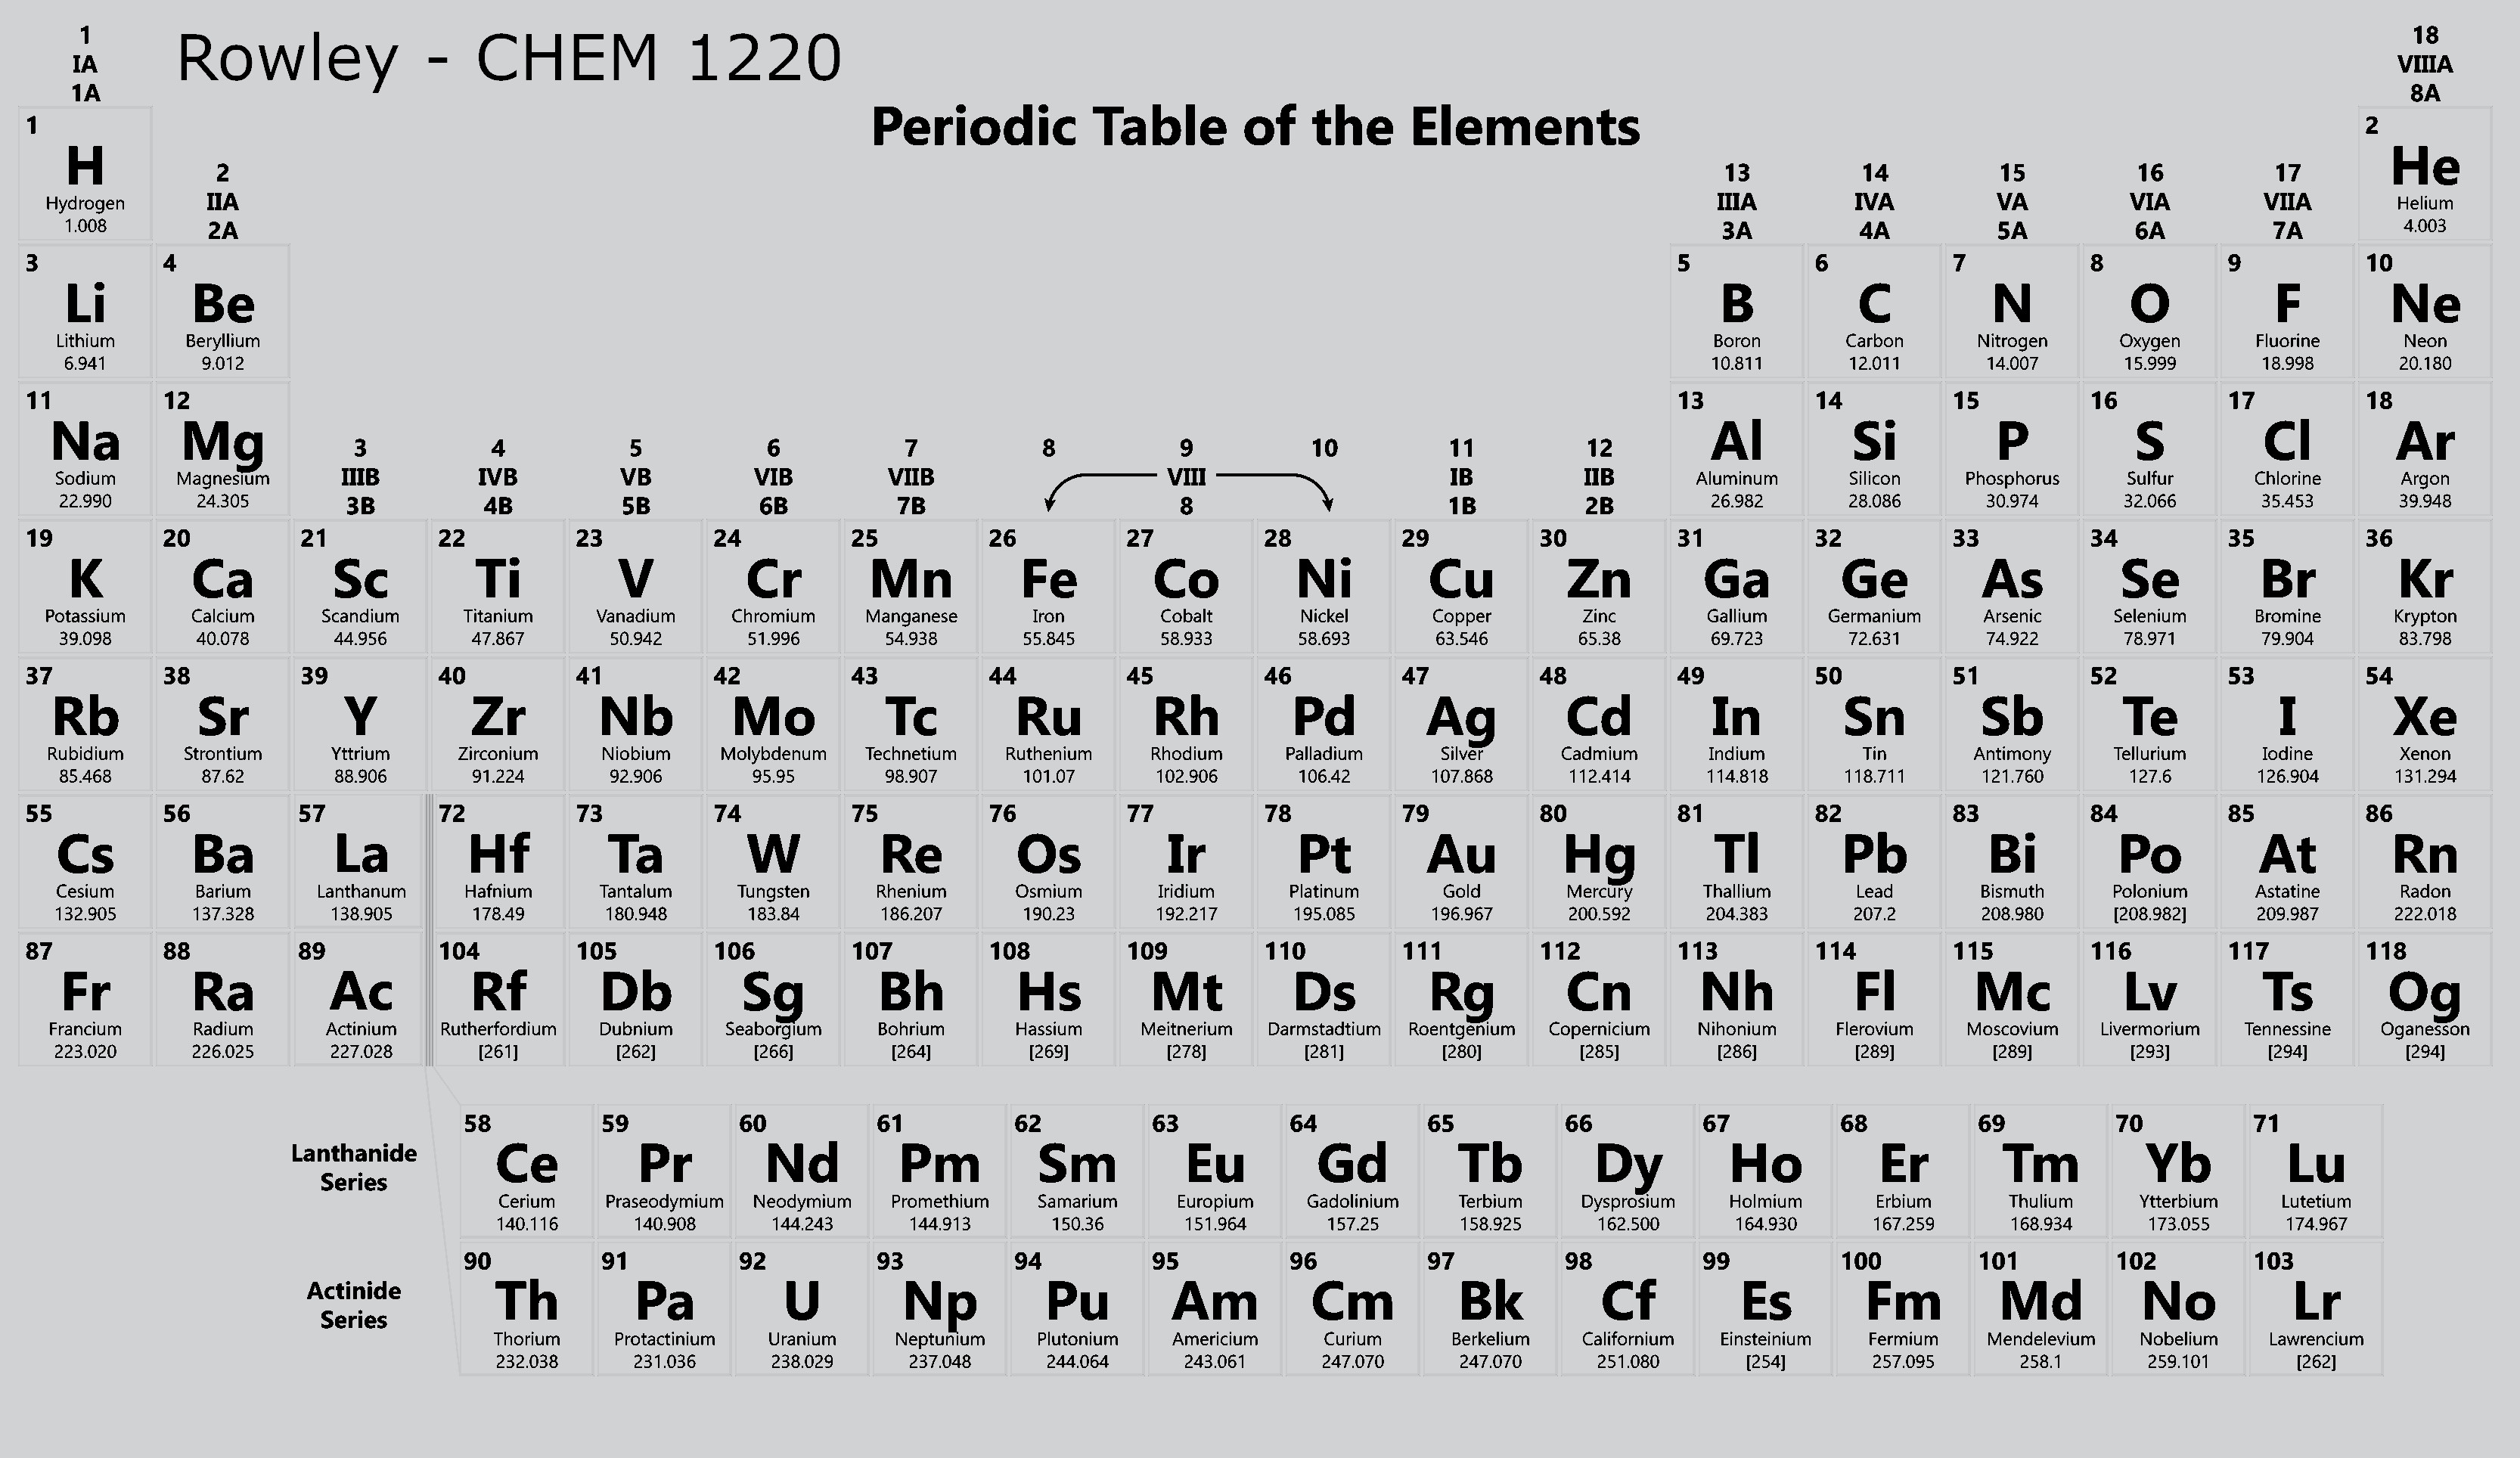
\includegraphics[width=1.3\textwidth, angle =90]{UpdatedTable}

	\restoregeometry

	
\end{document}